\documentclass[14pt, a4paper]{extarticle}

\usepackage{KrtchGOST}
\usepackage{hyperref}
\usepackage{listings}
\usepackage{array}
\usepackage{caption}
% \hypersetup
% {
% 	pdftex,
% 	colorlinks = true,
% 	linkcolor = red,
% 	filecolor = magenta,
% 	citecolor = green,      
% 	urlcolor = cyan,
% }


% к таблице и листингу подпись сверху, перед каждым иллюстративным материалом анонсировать
% написатьт в квадратных скобках к рекурсии комментарием что это метод и понятно почему вызываем его снова
\definecolor{mylightgray}{RGB}{240,240,240}
\definecolor{mygreen}{rgb}{0,0.6,0}
\definecolor{mygray}{rgb}{0.5,0.5,0.5}
\definecolor{mymauve}{rgb}{0.58,0,0.82}

\lstset
{
	backgroundcolor=\color{mylightgray},rulecolor=\color{red},  % choose the background color; you must add \usepackage{color} or \usepackage{xcolor}; should come as last argument
	basicstyle=\footnotesize\ttfamily,        % the size of the fonts that are used for the code
	breakatwhitespace=false,         % sets if automatic breaks should only happen at whitespace
	breaklines=true,                 % sets automatic line breaking
	captionpos=t,                    % sets the caption-position to bottom
	commentstyle=\color{mygreen},    % comment style
	extendedchars=false,              % lets you use non-ASCII characters; for 8-bits encodings only, does not work with UTF-8
	firstnumber=0,                % start line enumeration with line 1000
	frame=shadowbox,
	%rulesepcolor=\color{green},	                   % adds a frame around the code
	keepspaces=true,                 % keeps spaces in text, useful for keeping indentation of code (possibly needs columns=flexible)
	keywordstyle=\color{blue}\textbf,       % keyword style
	language=c++,                 % the language of the code
	morekeywords={*,...},            % if you want to add more keywords to the set
	numbers=left,                    % where to put the line-numbers; possible values are (none, left, right)
	numbersep=5pt,                   % how far the line-numbers are from the code
	numberstyle=\scriptsize\color{mygray}, % the style that is used for the line-numbers
	rulecolor=\color{black},         % if not set, the frame-color may be changed on line-breaks within not-black text (e.g. comments (green here))
	showspaces=false,                % show spaces everywhere adding particular underscores; it overrides 'showstringspaces'
	showstringspaces=false,          % underline spaces within strings only
	showtabs=false,                  % show tabs within strings adding particular underscores
	stepnumber=1,                    % the step between two line-numbers. If it's 1, each line will be numbered
	stringstyle=\color{mymauve},     % string literal style
	tabsize=4,	                   % sets default tabsize to 2 spaces
	title=\lstname                   % show the filename of files included with \lstinputlisting; also try caption instead of title
}
%\usepackage{YATPR}
\usepackage{float}

\restylefloat{table}

\begin{document}
\begin{titlepage}
	\newgeometry{pdftex, left=2cm, right=2cm, top=2.5cm, bottom=2.5cm}
	\fontsize{12pt}{12pt}\selectfont
	\noindent \begin{minipage}{0.15\textwidth}
		
\includegraphics[width=\linewidth]{pictures/b_logo.jpg}
	\end{minipage}
	\noindent\begin{minipage}{0.9\textwidth}\centering
		\textbf{Министерство науки и высшего образования Российской Федерации}\\
		\textbf{Федеральное государственное бюджетное образовательное учреждение высшего образования}\\
		\textbf{«Московский государственный технический университет имени Н.Э.~Баумана}\\
		\textbf{(национальный исследовательский университет)»}\\
		\textbf{(МГТУ им. Н.Э.~Баумана)}
	\end{minipage}
	
	\noindent\rule{18cm}{3pt}
	\newline\newline
	\noindent ФАКУЛЬТЕТ $\underline{\text{«Информатика и системы управления»}}$ \newline\newline
	\noindent КАФЕДРА $\underline{\text{«Программное обеспечение ЭВМ и информационные технологии»}}$\newline\newline\newline\newline\newline\newline\newline
	
	
	\begin{center}
		\Large\textbf{Отчёт по лабораторной работе №2 по курсу "Анализ алгоритмов"}\newline
	\end{center}
	
	\noindent\textbf{Тема} $\underline{\text{Алгоритмы умножения матриц}}$\newline\newline\newline
	\noindent\textbf{Студент} $\underline{\text{Михаил Коротыч~~~~~~~~~~~~~~~~~~~~~~~~~~~~~~~~~~~~~~~~~}}$\newline\newline
	\noindent\textbf{Группа} $\underline{\text{ИУ7-55Б~~~~~~~~~~~~~~~~~~~~~~~~~~~~~~~~~~~~~~~~~~~~~~~~~~}}$\newline\newline
	\noindent\textbf{Оценка (баллы)} $\underline{\text{~~~~~~~~~~~~~~~~~~~~~~~~~~~~~~~~~~~~~~~~~~~~~~~~~}}$\newline\newline
	\noindent\textbf{Преподаватели} $\underline{\text{Волкова Л.Л., Строганов Ю.В.~~~~~~~~~~~}}$\newline
	
	\begin{center}
		\vfill
		Москва~---~\the\year
		~г.
	\end{center}
 \restoregeometry
\end{titlepage}

\tableofcontents 
\newpage
\section*{Введение}
\addcontentsline{toc}{section}{Введение}
Термин «матрица» применяется во множестве разных областей: от программирования до кинематографии.

Матрица - это математический объект, представляющий из себя набор упорядоченных чисел (целых, дробных или даже комплексных). Эти числа записываются, как правило в виде квадратной или прямоугольной таблицы, над которой можно совершать различные операции. Матрицы — очень важный математический инструмент, позволяющий решать множество задач от систем уравнений до оптимизации поставок.

Мы встречаемся с матрицами каждый день, так как любая числовая информация, занесённая в таблицу, уже в какой-то степени считается матрицей.

Целью работы работы является изучение и реализация алгоритмов умножения матриц, вычисление трудоёмкости этих алгоритмов. В данной лабораторной работе рассматривается стандартный алгоритм умножения матриц, алгоритм Винограда и модифицированный алгоритм Винограда.

Для достижения цели ставятся следующие задачи:
\begin{itemize}
    \item изучить классический алгоритм умножения матриц, алгоритм Винограда и модифицированный алгоритм Винограда;
    \item сравнить классический алгоритм умножения матриц, алгоритм Винограда и модифицированный алгоритм Винограда;
    \item выявить достоинства и недостатки рассмотренных алгоритмов;
    \item дать оценку трудоёмкости алгоритмов;
    \item реализовать рассмотренные алгоритмы;
    \item замерить время работы алгоритмов;
    \item описать и обосновать полученные результаты в отчёте о выполненной лабораторной
работе. 
\end{itemize}

\newpage
\section{Аналитическая часть}
%\addcontentsline{toc}{section}{Аналитическая часть}

Матрица – математический объект, эквивалентный двумерному массиву. Числа располагаются в матрице по строкам и столбцам. Две матрицы одинакового размера можно поэлементно сложить или вычесть друг из друга \cite{matr}.

Если число столбцов в первой матрице совпадает с числом строк во второй, то эти две матрицы можно перемножить. У произведения будет столько же строк, сколько в первой матрице, и столько же столбцов, сколько во второй. При умножении матрицы размером $3 \times 4$ на матрицу размером $4 \times 7$ мы получаем матрицу размером $3 \times 7$. Умножение матриц некоммутативно: оба произведения $AB$ и $BA$ двух квадратных матриц одинакового размера можно вычислить, однако результаты, вообще говоря, будут отличаться друг от друга \cite{matr}.

\subsection{Классический алгоритм умножения матриц}

Пусть даны две прямоугольные матрицы А (\ref{bmtr:matrixa}) и В (\ref{bmtr:matrixb}) размерности m на n и n на l соответсвенно: 
\begin{equation}
 \label{bmtr:matrixa}
\begin{bmatrix}
a_{1,1} & ... & a_{1,n} \\
... & ... & ... \\
a_{m,1} & ... & a_{m,n} \\
\end{bmatrix} \\
\end{equation}

\begin{equation}
 \label{bmtr:matrixb}
\begin{bmatrix}
b_{1,1} & ... & b_{1,l} \\
... & ... & ... \\
b_{n,1} & ... & b_{n,l} \\
\end{bmatrix} \\
\end{equation}

В результате получим матрицу C \ref{bmtr:matrixc} размерности m на l:
	
\begin{equation}
 \label{bmtr:matrixc}
\begin{bmatrix}
c_{1,1} & ... & c_{1,l} \\
... & ... & ... \\
c_{m,1} & ... & c_{m,l} \\
\end{bmatrix} \\
\end{equation}

Формула \ref{bmtr:cij} - формула расчёта элемента, находящегося на i-ой строке j-ого столбца матрицы C:

\begin{equation}
 \label{bmtr:cij}
c_{i,j} = \sum\limits_{r=1}^n a_{i,r}\cdot b_{r,j}
\end{equation}

\subsection{Алгоритм Винограда}
Если посмотреть на результат умножения двух матриц, то видно, что каждый элемент в нём представляет собой скалярное произведение соответствующих строки и столбца исходных матриц. Можно заметить также, что такое умножение допускает предварительную обработку, позволяющую часть работы выполнить заранее ~\cite{vinogr}.
 
Рассмотрим два вектора $V = (v1, v2, v3, v4)$ и $W = (w1, w2, w3, w4)$. Их скалярное произведение ~\ref{eq:dot} равно: 

\begin{equation}
 \label{eq:dot}
 V \cdot W=v_1 \cdot w_1 + v_2 \cdot w_2 + v_3 \cdot w_3 + v_4 \cdot w_4\\
\end{equation}


Это равенство можно переписать в виде \ref{eq:dot1}:

\begin{equation}
 \label{eq:dot1}
V \cdot W=(v_1 + w_2) \cdot (v_2 + w_1) + (v_3 + w_4) \cdot (v_4 + w_3) - v_1 \cdot v_2 - 
v_3 \cdot v_4 - w_1 \cdot w_2 - w_3 \cdot w_4
\end{equation}

Менее очевидно, что выражение в правой части последнего равенства допускает предварительную обработку: его части можно вычислить заранее и запомнить для каждой строки первой матрицы и для каждого столбца второй. 
Это означает, что над предварительно обработанными элементами нам придётся выполнять лишь первые два умножения и последующие пять сложений, а также дополнительно два сложения ~\cite{vinogr}. 

\subsection{Оптимизированный алгоритм Винограда}
Оптимизированный алгоритм Винограда представляет собой обычный алгоритм Винограда, за исключением следующих оптимизаций:

\begin{itemize}
    \item вычисление происходит заранее;
    \item используется битовый сдвиг вместо деления на 2;
    \item последний цикл для нечётных элементов включён в основной цикл, используя дополнительные операции в случае нечётности N.
\end{itemize}

\subsection{Вывод}
Были рассмотрены алгоритмы классического умножения матриц и алгоритм Винограда, основная разница которого - наличие предварительной обработки, а также уменьшение количества операций умножения.

\newpage
\section{Конструкторская часть}

\subsection{Схемы алгоритмов}
На рисунке \ref{fig:base} представлена схема классического умножения матриц.

\newpage
\begin{figure}
\center{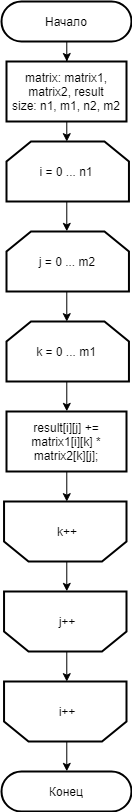
\includegraphics[height=155mm]{pictures/base.png}}
\caption{Схема классического алгоритма умножения матриц}
\label{fig:base}
\end{figure}

На рисунках \ref{fig:vin1}, \ref{fig:vin2}, \ref{fig:vin3}, \ref{fig:vin4} представлена схема алгоритма умножения матриц Винограда.

\begin{figure}
\center{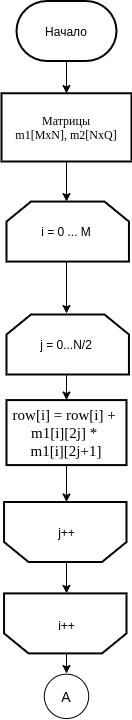
\includegraphics[scale=0.8]{pictures/vin1.png}}
\caption{Схема алгоритма Винограда (часть 1)}
\label{fig:vin1}
\end{figure}

\begin{figure}
\center{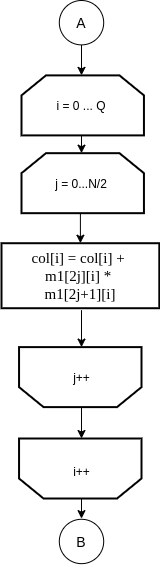
\includegraphics[scale=1]{pictures/vin2.png}}
\caption{Схема алгоритма Винограда (часть 2)}
\label{fig:vin2}
\end{figure}

\begin{figure}
\center{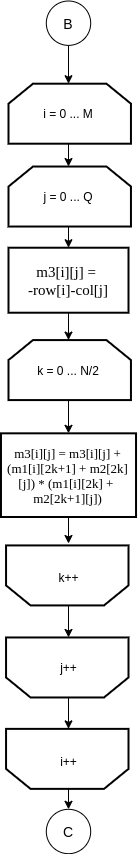
\includegraphics[scale=0.8]{pictures/vin3.png}}
\caption{Схема алгоритма Винограда (часть 3)}
\label{fig:vin3}
\end{figure}

\begin{figure}
\center{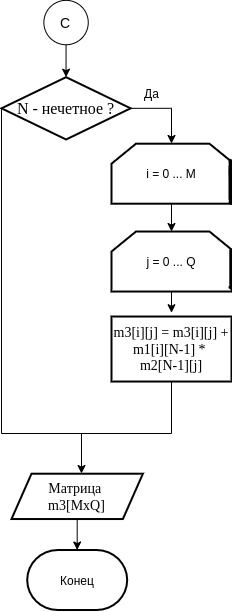
\includegraphics[scale=0.8]{pictures/Inkedvin4_LI.jpg}}
\caption{Схема алгоритма Винограда (часть 4)}
\label{fig:vin4}
\end{figure}

\newpage
На рисунках \ref{fig:vinOpt1}, \ref{fig:vinOpt2}, \ref{fig:vinOpt3}, \ref{fig:vinOpt4} представлена схема оптимизированного алгоритма умножения матриц Винограда.

\begin{figure}
\center{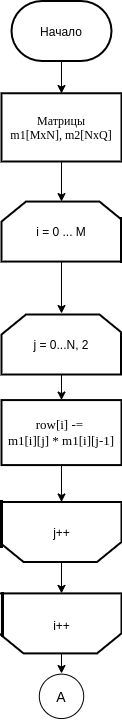
\includegraphics[scale=0.8]{pictures/vinopt1.png}}
\caption{Схема оптимизированного алгоритма Винограда(часть 1)}
\label{fig:vinOpt1}
\end{figure}

\begin{figure}
\center{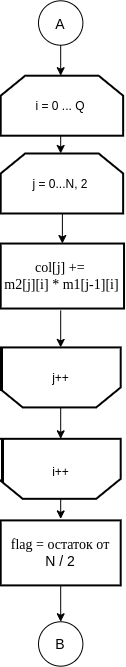
\includegraphics[scale=1]{pictures/vinopt2.png}}
\caption{Схема оптимизированного алгоритма Винограда(часть 2)}
\label{fig:vinOpt2}
\end{figure}

\begin{figure}
\center{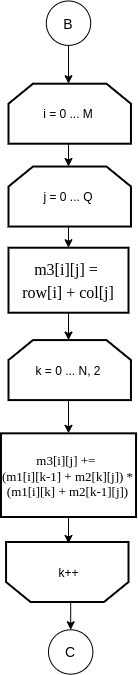
\includegraphics[scale=0.95]{pictures/vinopt3.png}}
\caption{Схема оптимизированного алгоритма Винограда(часть 3)}
\label{fig:vinOpt3}
\end{figure}

\begin{figure}
\center{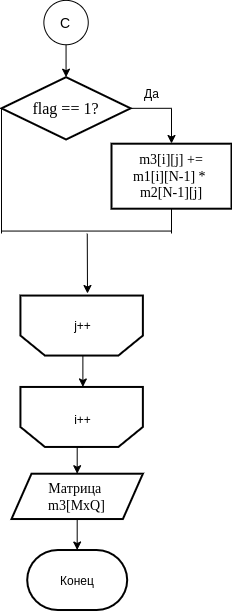
\includegraphics[scale=0.9]{pictures/vinopt4.png}}
\caption{Схема оптимизированного алгоритма Винограда(часть 4)}
\label{fig:vinOpt4}
\end{figure}

\newpage
\subsection{Вычисление трудоёмкости алгоритма}
Введём модель трудоёмкости для оценки алгоритмов.
\begin{enumerate}
  	\item Базовые операции стоимостью 1: +, -, *, /, =, ==, <=, >=, !=, +=, [], получение полей класса.
	\item Оценка трудоёмкости цикла: 
	
	f\_цикла = f\_инициализации + f\_сравнения + N * (f\_инкремента + f\_сравнения + f\_тела).
	
	\item Стоимость условного перехода возьмём за 0, стоимость вычисления условия остаётся. В условном операторе может возникнуть лучший и худший случаи по трудоёмкости в зависимости от выполнения условия и в зависимости от входных данных алгоритма.
\end{enumerate}

\subsection{Оценка трудоёмкости алгоритмов умножения матриц}
%\hfill
Оценка трудоёмкости дана согласно введённой выше модели вычислений.

\begin{enumerate}
	\item Стандартный алгоритм
	
	$$f=2+M(2+2+Q(2+2+N(2+8+1+1+1)))=13 \cdot$$
	$$\cdot MNQ+4MQ+4M+2 \approx 13 \cdot MNQ$$ 
		
    \item Алгоритм Винограда
        \begin{enumerate}
            \item Трудоёмкость алгоритма Винограда:\\
            \item Первый цикл: $\frac{15}{2} \cdot N  Q + 5 \cdot M + 2$ \\
            Второй цикл: $\frac{15}{2} \cdot M  N + 5 \cdot M + 2$\\
            Третий цикл: $13 \cdot M  N Q + 12 \cdot M Q + 4 \cdot M + 2$\\
            \item Условный переход:
            
            $\begin{bmatrix}
            2    &&, \text{лучший случай при чётном N}\\
            15 \cdot QM + 4 \cdot M + 4 &&, \text{худший случай}\\
            \end{bmatrix} $ \\
            \item Итого:
            
            $f = \frac{15}{2} \cdot M  N + \frac{15}{2} \cdot Q  N + 9 \cdot M + 8 +  5 \cdot Q + 13 \cdot M  N Q + 12 \cdot M Q +
            \begin{bmatrix}
            2    &&, \text{в лучшем случае}\\
            15 \cdot QM + 4 \cdot M + 4 &&, \text{в худшем случае}\\
            \end{bmatrix} $ \\
            $$f \approx 13 \cdot MNQ $$
        \end{enumerate}

    \item Оптимизированный алгоритм Винограда

        Введём оптимизации:
		\begin{enumerate}
		    \item замена оперции = на += или -=;
		    \item избавление от деления в условиях цикла (j < N, j += 2);
			\item заносение проверки на нечётность количества строк внутрь основных циклов;
			\item расчёт условия для последнего цикла один раз, а далее использование флага;
		\end{enumerate}
			
        Первый цикл: $4 \cdot N  Q + 4 \cdot M + 2$ \\
        Второй цикл: $4 \cdot M  N + 4 \cdot M + 2$\\
        Третий цикл: $9 \cdot M  N Q + 10 \cdot M Q + 4 \cdot M + 2$\\
        Условный переход:

        $\begin{bmatrix}
            2   &&, \text{лучший случай (при четном N)}\\
            10 \cdot QM &&, \text{худший случай}\\
        \end{bmatrix} $ \\

        Трудоёмкость оптимизированного алгоритма Винограда:
        \\$$f = 4 \cdot N  Q + 4 \cdot M + 2 + 4 \cdot M  N + 4 \cdot M + 2 + 9 \cdot M  N Q + 10 \cdot M Q + 4 \cdot M + 2 + $$
        $$ + \begin{bmatrix}
                    2   &&, \text{л.c}\\
                    10 \cdot QM &&, \text{х.c}\\
            \end{bmatrix} \approx 9 \cdot MNQ$$
	\end{enumerate}

\subsection{Вывод}
На основе теоретических данных, полученных из аналитического раздела были построены схемы требуемых алгоритмов и вычислены их трудоёмкости.

\newpage
\section{Технологическая часть}

\subsection{Требования к вводу}
На вход подаются две матрицы. Операция умножения двух матриц выполнима только в том случае, если число столбцов в первом сомножителе равно числу строк во втором; в этом случае говорят, что матрицы согласованы.

\subsection{Требования к выводу}
Матрица (результат умножения матриц, поданых на вход).

\subsection{Требования к программе}
Две пустые матрицы - корректный ввод. Программа не должна аварийно завершаться.

\subsection{Выбор языка программирования}
Языком программирования был выбран C++.

Время работы алгоритмов было замерено с помощью функции GetCPUTime из <Windows.h>.

\subsection{Сведения о модулях программы}
Программа состоит из модуля main.cpp. В модуле main одна за другой вызываются подпрограммы каждого рассматриваемого алгоритма, а также подпрограммы подготови к использыванию этих алгоритмов, например создание и инициализация матриц.

На листингах \ref{lst:base}, \ref{lst:vin}, \ref{lst:vin_opt} представлен код алгоритмов.
\begin{lstlisting}[label=lst:base,caption=Классический алгоритм умножения матриц]
my_matrix classical_multiplication(my_matrix matrix1, my_matrix matrix2)
{
	my_matrix result
	{
		std::vector<std::vector<float>>(matrix1.n, std::vector<float>(matrix2.m, 0)),
		matrix1.n,
		matrix2.m
	};

	for (int i = 0; i < result.n; i++)
		for (int j = 0; j < result.m; j++)
			for (int k = 0; k < matrix1.m; k++)
				result.values[i][j] += matrix1.values[i][k] * matrix2.values[k][j];

	return result;
}
 \end{lstlisting}
 
\newpage
\begin{lstlisting}[label=lst:vin,caption=Алгоритм Винограда]
	my_matrix result
	{
		std::vector<std::vector<float>>(matrix1.n, std::vector<float>(matrix2.m, 0)),
		matrix1.n,
		matrix2.m
	};

	std::vector<float> row(matrix1.n, 0);
	for (int i = 0; i < matrix1.n; i++)
		for (int j = 0; j < matrix1.m / 2; j++)
			row[i] += matrix1.values[i][2 * j] * matrix1.values[i][2 * j + 1];

	std::vector<float> column(matrix2.m, 0);
	for (int i = 0; i < matrix2.m; i++)
		for (int j = 0; j < matrix1.m / 2; j++)
			column[i] += matrix2.values[2 * j][i] * matrix2.values[2 * j + 1][i];

	for (int i = 0; i < matrix1.n; i++)
		for (int j = 0; j < matrix2.m; j++)
		{
			result.values[i][j] = -row[i] - column[j];
			for (int k = 0; k < matrix1.m / 2; k++)
				result.values[i][j] += (matrix1.values[i][2 * k + 1] + matrix2.values[2 * k][j]) * (matrix1.values[i][2 * k] + matrix2.values[2 * k + 1][j]);
		}

	if (matrix1.m % 2)
		for (int i = 0; i < matrix1.n; i++)
			for (int j = 0; j < matrix2.m; j++)
				result.values[i][j] += matrix1.values[i][matrix1.m - 1] * matrix2.values[matrix1.m - 1][j];

	return result;
}
\end{lstlisting}
 
\newpage
  \begin{lstlisting}[label=lst:vin_opt,caption=Оптимизированный алгоритм Винограда]
my_matrix optimized_winograd_algorithm(my_matrix matrix1, my_matrix matrix2)
{
	my_matrix result
	{
		std::vector<std::vector<float>>(matrix1.n, std::vector<float>(matrix2.m, 0)),
		matrix1.n,
		matrix2.m
	};

	std::vector<float> row(matrix1.n, 0);
	for (int i = 0; i < matrix1.n; i++)
		for (int j = 1; j < matrix1.m; j += 2)
			row[i] -= matrix1.values[i][j] * matrix1.values[i][j - 1];

	std::vector<float> column(matrix2.m, 0);
	for (int i = 0; i < matrix2.m; i++)
		for (int j = 1; j < matrix1.m; j += 2)
			column[i] -= matrix2.values[j][i] * matrix2.values[j - 1][i];

	for (int i = 0; i < matrix1.n; i++)
		for (int j = 0; j < matrix2.m; j++)
		{
			result.values[i][j] += row[i] + column[j];
			for (int k = 1; k < matrix1.m; k += 2)
			{
				result.values[i][j] += (matrix1.values[i][k - 1] + matrix2.values[k][j]) * (matrix1.values[i][k] + matrix2.values[k - 1][j]);
				if (matrix1.m % 2)
					result.values[i][j] += matrix1.values[i][matrix1.m - 1] * matrix2.values[matrix1.m - 1][j];
			}
		}

	return result;
}
 \end{lstlisting}

\newpage
\subsection{Функциональные тесты}
	\begin{center}
	      Таблица 3.1 -- Функциональные тесты
	\end{center}
\begin{table}[H]
\label{tabular:functional_test}
 \begin{center}
\begin{tabular}{ | c | c | c | c |}
			\hline
			% {\centering GallusGallus \\ CC \\ t = 104}
			\textbf{Матрица1} & \textbf{Матрица2} & \multicolumn{1}{|p{3cm}|}{\textbf{Ожидаемый результат}} & \multicolumn{1}{|p{3cm}|}{\textbf{Фактический результат}}\\ \hline
			$\begin{bmatrix} 
   			1&2&3 \\
    			4&5&6 \\ 
   			7&8&9 \\ 
			\end{bmatrix}$ & 
			$\begin{bmatrix} 
   			1&2&3 \\
    			4&5&6 \\ 
   			7&8&9 \\ 
			\end{bmatrix}$ &
			$\begin{bmatrix} 
   			30&36&42 \\
    			66&81&96 \\ 
   			102&126&150 \\ 
			\end{bmatrix} $ &
			$\begin{bmatrix} 
   			30&36&42 \\
    			66&81&96 \\ 
   			102&126&150 \\ 
			\end{bmatrix} $\\
			\hline

			
			$\begin{bmatrix} 
   			1&1&1 \\
    			1&1&1 \\ 
   			1&1&1 \\ 
			\end{bmatrix}$ & 
			$\begin{bmatrix} 
   			1&1&1 \\
    			1&1&1 \\ 
			\end{bmatrix}$ &
			$\begin{matrix} 
   			\text{Матрицы не могут} \\
    			\text{быть перемножены} \\ 
			\end{matrix} $ &
			$\begin{matrix} 
   			\text{Матрицы не могут} \\
    			\text{быть перемножены} \\ 
			\end{matrix} $ \\
			\hline
			
			$\begin{bmatrix} 
   			1&2 \\
    			3&4 \\ 
   			5&6 \\ 
			\end{bmatrix}$ & 
			$\begin{bmatrix} 
   			1&2&3 \\
    			4&5&6 \\ 
			\end{bmatrix}$ &
			$\begin{bmatrix} 
   			9&12&15 \\
    			19&26&33 \\ 
   			29&40&51 \\ 
			\end{bmatrix} $ &
			$\begin{bmatrix} 
   			9&12&15 \\
    			19&26&33 \\ 
   			29&40&51 \\ 
			\end{bmatrix} $ \\
			\hline
		\end{tabular}
		
 \end{center}
\end{table} 

Все реализации алгоритмов на практике показали ожидаемый результат.

\subsection{Вывод}

В этом разделе была представлена реализация алгоритмов классического умножения матриц, алгоритма Винограда, оптимизирвоанного алгоритма Винограда. Тестирование показало, что алгоритмы реализованы правильно и работают корректно.

\newpage
\section{Исследовательская часть}

\subsection{Технические характеристики}
Технические характеристики устройства, на котором выполнялось тестирование, следующие:
\begin{itemize}
    \item Операционная система: Windows 10 64-bit;
    \item Память 8 ГБ;
    \item Процессор: Intel(R) Core(TM) i7-8550U CPU @ 1.80GHz   1.99 GHz.
\end{itemize}

\subsection{Демонстрация работы программы}
На рисунке \ref{fig:program} представлен результат работы программы.

\begin{figure}[H]
\center{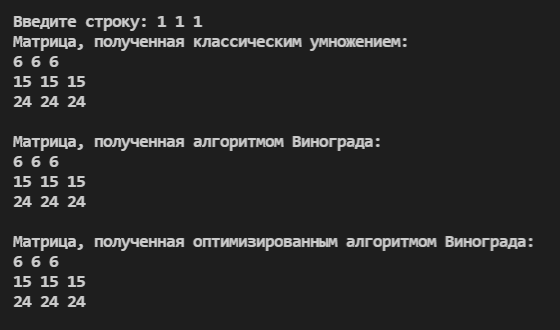
\includegraphics[scale=0.9]{pictures/program.png}}
\caption{Результат работы программы.}
\label{fig:program}
\end{figure}

\newpage
\subsection{Время работы алгоритмов}

Бал проведён замер времени работы из алгоритмов. Каждый замер времени проводился 10 раз и результат усреднялся. Первый эксперимент производится для лучшего случая на матрицах размерами от 100 на 100 до 500 на 500 с шагом 100. Рисунок \ref{fig:t_even}.

\begin{figure}[H]
\center{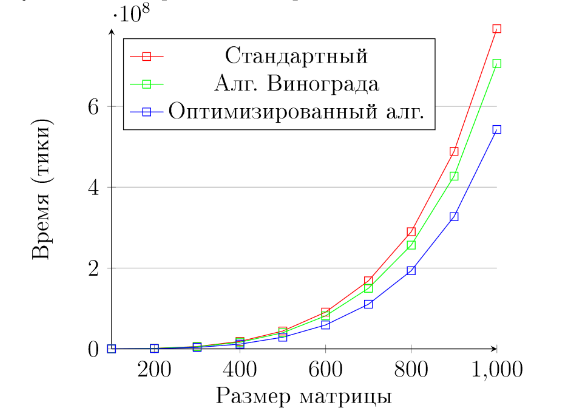
\includegraphics[scale=0.7]{pictures/lag1.png}}
\caption{Замеры времени на чётном количестве строк и столбцов квадратных матриц.}
\label{fig:t_even}
\end{figure}

Второй эксперимент производится для худшего случая, когда заданы матрицы с нечётными размерами от 101 на 101 до 501 на 501 с шагом 100. Рисунок \ref{fig:t}.

\begin{figure}[H]
\center{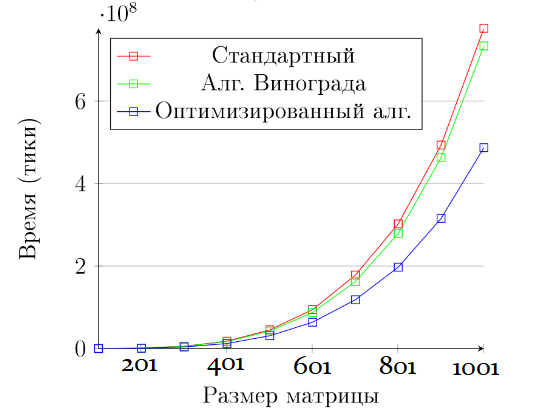
\includegraphics[scale=0.7]{pictures/alg2.png}}
\caption{Замеры времени на нечётном количестве строк и столбцов квадратных матриц.}
\label{fig:t}
\end{figure}

По результатам тестирования, все рассматриваемые алгоритмы реализованы правильно. Самым медленным оказался алгоритм классического умножения матриц, самым быстрым - оптимизированный алгоритм Винограда.

\subsection{Вывод}
В данном разделе протестированы алгоритмы умножения матриц. Классический алгоритм показал худшие результаты, что и следовало ожидать. Оптимизированный алгоритм Винограда проявил себя лучше остальных. Экспериментально было подтверждено различие по временной эффективности алгоритмов умножения матриц на материале замеров процессорного времени выполнения реализации на варьирующихся размерах матриц. Так, самым быстрым является оптимизированный алгоритм Винограда, на размере матрицы 400 на 400 он работает в 1,3 раза быстрее алгоритма Винограда без оптимизации и в 1,23 раз быстрее классического алгоритма умножения. Алгоритмы Винограда и классического умножения примерно сопоставимы.

\newpage
\section{Заключение}
Цель лабораторной работы достигнута. В ходе выполнения работы решены следующие задачи:
\begin{itemize}
    \item изучены классический алгоритм умножения матриц, алгоритм Винограда и модифицированный алгоритм Винограда;
    \item реализованы классический алгоритм умножения матриц, алгоритм Винограда и модифицированный алгоритм Винограда;
    \item дана оценка трудоёмкости алгоритмов;
    \item замерено время работы алгоритмов;
    \item описаны и обоснованы полученные результаты в отчёте о выполненной лабораторной
работе.
\end{itemize}

Экспериментально было подтверждено различие по временной эффективности алгоритмов умножения матриц на материале замеров процессорного времени выполнения реализации на варьирующихся размерах матриц. Так, самым быстрым является оптимизированный алгоритм Винограда, на размере матрицы 400 на 400 он работает в 1,3 раза быстрее алгоритма Винограда без оптимизации и в 1,23 раз быстрее классического алгоритма умножения. Алгоритмы Винограда и классического умножения примерно сопоставимы.

На основании сравнения данных алгоритмов был сделан вывод, что классический алгоритм является более эффективным, чем алгоритм Винограда, однако после ряда оптимизаций алгоритм Винограда становится значительно быстрее классического. 

\newpage
\section*{Список литературы}
\addcontentsline{toc}{section}{Список литературы}

[1] Умножение матриц.[Электронный ресурс]. Режим доступа: https://life-prog.ru/2\_90314\_umnozhenie-matrits.html
 	    
[2] Умножение матриц по Винограду [Электронный ресурс]. Режим доступа: http://algolib.narod.ru/Math/Matrix.html
 	    
[3] CPP Reference [Электронный ресурс]. Режим доступа: https://en.cppreference.com/w/

[4] Процессор Intel Соrе 17-85500 [Электронный ресурc] Режим доступа: https://ark.intel.com/content/www/ru/ru/ark/products/122589/intel-core-i7-8550u-processor-8m-cache-up-to-4-00-ghz.html

[5] Windows 10 [Электронный ресурc] Режим доступа: https://www.microsoft.com/ru-ru/windows/get-windows-10

\end{document}